
\section{Equations for incompressible fluids}

FIXME: lay out theory e.g.~from \citep{Acheson1990,Ockendonetal2003}

FIXME in this section our notation hits a bit of an ``subscripting crisis'', so in this section we write for the velocity field
    $$\bu = \left<u^x,u^y,u^z\right>$$
so that superscript denotes component

The incompressible variable-viscosity Navier-Stokes has these main equations
\begin{align}
\rho \left(\frac{\partial \bu}{\partial t} + \bu \cdot \grad \bu\right) &= \Div \sigma + \bg \label{eq:ok:stokesgeneralconserve} \\
\sigma &= 2 \nu\, D \bu - p I \label{eq:ok:stokesgenerallaw} \\
\Div \bu &= 0 \label{eq:ok:stokesgeneralincomp}
\end{align}
where
\begin{equation}
\grad \bu = \renewcommand{\arraystretch}{1.3}\begin{bmatrix}
    \frac{\partial u^x}{\partial x} & \frac{\partial u^y}{\partial x} & \frac{\partial u^z}{\partial x} \\
    \frac{\partial u^x}{\partial y} & \frac{\partial u^y}{\partial y} & \frac{\partial u^z}{\partial y} \\
    \frac{\partial u^x}{\partial z} & \frac{\partial u^y}{\partial z} & \frac{\partial u^z}{\partial z}
    \end{bmatrix}  \label{eq:ok:gradudefinition}
\end{equation}
and
    $$D \bu = \frac{1}{2} \left(\grad \bu + \grad \bu^{\top}\right).$$

FIXME: theory where Froude $\approx 0$

The variable-viscosity Stokes equations, in terms of velocity, are
\begin{align*}
- \Div \left(\nu \left(\grad \bu + \grad \bu^{\top}\right)\right) + \grad p &= \bg \\
\Div \bu &= 0
\end{align*}

We will, however, first consider the case where the viscosity $\nu=1$ is constant.  In such case the velocity second derivative term can be simplified, and recognized as an application of the Laplacian operator (Exercise \ref{chap:ok}.\ref{exer:ok:constantviscositystokes}).  For this Chapter the Stokes equations are
\begin{align}
- \grad^2 \bu + \grad p &= \bg  \label{eq:ok:constantviscositystokes} \\
\Div \bu &= 0  \label{eq:ok:constantviscosityincomp}
\end{align}
This is a Poisson-like problem for $\bu$, but with pressure as an additional unknown and with an additional equation stating incompressiblity.  Note that body force and the pressure gradient are together balanced by the viscous stresses. 


\section{Weak form of the Stokes equations}

FIXME: theory from \citep{Braess2007,Elmanetal2005}; derive quickly by multiplying \eqref{eq:ok:constantviscositystokes}--\eqref{eq:ok:constantviscosityincomp} by test functions and integrating

FIXME assume $\bu=\bu_D$ (known) on $\partial_D\Omega$.  restrict to $\partial \bu/\partial n - \bn p = 0$ on $\partial_N\Omega$; i.e.~arbitrary Dirichlet but homogeneous Neumann; contrast \citep{Elmanetal2005}

If $\bu \in W_D^{1,2}(\Omega)^3$ and $p \in L^2(\Omega)$ solves
\begin{align}
\int_\Omega \grad \bu \,:\, \grad \bv - p \Div \bv &= \int_\Omega \bg \cdot \bv \label{eq:ok:weakstokesvelocity} \\
\int_\Omega q \Div \bu &= 0 \label{eq:ok:weakstokespressure}
\end{align}
for all $\bv \in W_0^{1,2}(\Omega)^3$ and $q \in L^2(\Omega)$ then we say $\bu,p$ solve the \emph{weak form of the Stokes} equations.  For clarity, in the 2D case the product of velocity gradients is
     $$\grad \bu \,:\, \grad \bv = \grad u^x \cdot \grad v^x + \grad u^y \cdot \grad v^y.$$


\section{A small example step \dots in the wrong direction}

FIXME: dimension 8 problem from using $\bu\in Q^1$ and $p\in P^0$ on 4-element mesh; goal of this example is to show how inf-sup condition relates to linear independence of constraints

We consider a ``Poiseuille flow'' \citep{Elmanetal2005} in 2D on $\Omega=(-1,1)\times(-1,1)$ with no body force so $\bg=0$.  On the top and bottom we have homogeneous Dirichlet boundary conditions $\bu=\left<0,0\right>$.  On the left side we have Dirichlet inflow boundary conditions $\bu(-1,y) = \left<1-y^2,0\right>$.  On the right side we have a Neumann stress-free boundary condition $\partial \bu/\partial n - \bn p = 0$, noting $\bn = \left<1,0\right>$.

\newcommand{\one}{{\large \mathbb{1}}}

This small example will help us think.  We have nine total nodes and four elements ($\square_k$) as in Figure \ref{fig:ok:poiseuille}.

\begin{figure}
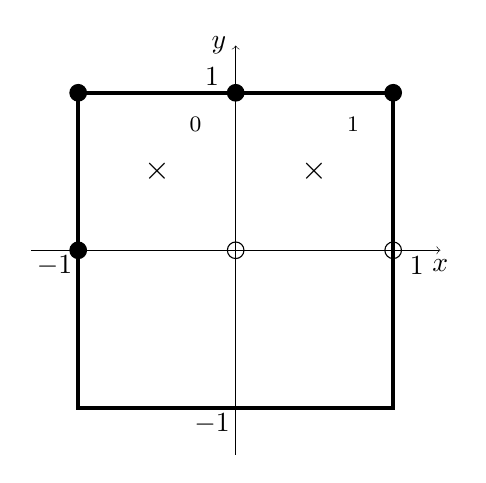
\begin{tikzpicture}[scale=2.0]
% origin of axes at (0.0,0.0) and square has half-width 1.0
  \draw[->,very thin] (-1.3,0.0) -- (1.3,0.0) node[below] {$x$};
  \draw[->,very thin] (0.0,-1.3) -- (0.0,1.3) node[left] {$y$};
  \draw[line width=1.5pt] (-1,-1) -- (1,-1) -- (1,1) -- (-1,1) -- cycle;
  \node at (1.15,-0.1) {$1$};
  \node at (-1.15,-0.1) {$-1$};
  \node at (-0.15,1.1) {$1$};
  \node at (-0.15,-1.1) {$-1$};
  \node at (-0.25,0.8) {\large $\square_0$};
  \node at (0.75,0.8) {\large $\square_1$};
  \draw (0.0,0.0) circle (1.5pt);
  \draw (1.0,0.0) circle (1.5pt);
  \filldraw (-1.0,0.0) circle (1.5pt);
  \filldraw (-1.0,1.0) circle (1.5pt);
  \filldraw (0.0,1.0) circle (1.5pt);
  \filldraw (1.0,1.0) circle (1.5pt);
  \node at (-0.5,0.5) {\large $\times$};
  \node at (0.5,0.5) {\large $\times$};
  %\filldraw (0.5,0.5) circle (1.0pt) node[xshift=6mm,yshift=2mm] {$foo$};
\end{tikzpicture}


\caption{$\Omega=(-1,1)\times(-1,1)$ for Poiseuille flow, with a very-coarse grid of four elements $\square_k$.  Open circles ``{\large $\circ$}'' are velocity unknowns, ``$\bullet$'' are Dirichlet boundary conditions, and ``$\times$'' are pressure unknowns.}
\label{fig:ok:poiseuille}
\end{figure}

Six of the nodes correspond to homogeneous Dirichlet boundary conditions on the velocity.  The single non-homogeneous Dirichlet boundary condition, at location $(-1,0)$, is incorporated into the solution by the expression
\begin{equation} 
\bu = \left<\psi_{-1}+\alpha_0\psi_0+\alpha_1\psi_1,\beta_0\psi_0+\beta_1\psi_1\right>  \label{eq:ok:smallexpansionvelocity}
\end{equation}
where $\psi_{-1},\psi_0,\psi_1$ denote $Q^1$ hat functions at points $(-1,0),(0,0),(1,0)$, respectively, and $\alpha_0,\alpha_1,\beta_0,\beta_1$ are unknown scalars.  (Because the boundary data is interpolated, the trial function space is only approximately inside the solution space $W_D^{1,2}(\Omega)^2$ for the continuous problem.)

The pressure solution is in terms of $P^0$ basis functions, which are characteristic functions on the elements $\one_j = \one_{\square_j}$, so
\begin{equation}
p = \gamma_0 \one_0 + \gamma_1 \one_1 + \gamma_2 \one_2 + \gamma_3 \one_3.  \label{eq:ok:smallexpansionpressure}
\end{equation}

Inserting \eqref{eq:ok:smallexpansionvelocity} and \eqref{eq:ok:smallexpansionpressure} into \eqref{eq:ok:weakstokesvelocity} gives
\begin{align}
&\alpha_0 \int_\Omega \grad \psi_0 \cdot \grad v^x + \beta_0 \int_\Omega \grad \psi_0 \cdot \grad v^y \label{eq:ok:smallconcretevelocity} \\
&\qquad + \alpha_1 \int_\Omega \grad \psi_1 \cdot \grad v^x + \beta_1 \int_\Omega \grad \psi_1 \cdot \grad v^y \notag \\
&\qquad - \gamma_0 \int_{\square_0} \Div \bv - \gamma_1 \int_{\square_1} \Div \bv - \gamma_2 \int_{\square_2} \Div \bv - \gamma_3 \int_{\square_3} \Div \bv \notag \\
&= - \int_\Omega \grad \psi_{-1} \cdot \grad v^x \notag
\end{align}
for test functions $\bv \in W_0^{1,2}(\Omega)^2$.  Inserting \eqref{eq:ok:smallexpansionvelocity} into \eqref{eq:ok:weakstokespressure}, and changing the sign to give symmetry (see below), gives
\begin{align}
&- \alpha_0 \int_\Omega q \frac{\partial \psi_0}{\partial x} - \beta_0 \int_\Omega q \frac{\partial \psi_0}{\partial y} - \alpha_1 \int_\Omega q \frac{\partial \psi_1}{\partial x} - \beta_1 \int_\Omega q \frac{\partial \psi_1}{\partial y}  \label{eq:ok:smallconcretepressure} \\
&= \int_\Omega q \frac{\partial \psi_{-1}}{\partial x} \notag
\end{align}
for test functions $q \in L^2(\Omega)$.

There are eight unknown scalars in system \eqref{eq:ok:smallconcretevelocity}, \eqref{eq:ok:smallconcretepressure}, namely $\alpha_j,\beta_j,\gamma_j$.  We choose velocity test functions from the basis of $Q^1$ hat functions at $(0,0),(1,0)$, so
\begin{equation}
\bv_i \in \left\{\left<\psi_0,0\right>, \left<0,\psi_0\right>, \left<\psi_1,0\right>, \left<0,\psi_1\right>\right\},  \label{eq:ok:smallvelocitytest}
\end{equation}
and pressure test functions from a $P^0$ basis,
\begin{equation}
q_i \in \{\one_0,\one_1,\one_2,\one_3\}.  \label{eq:ok:smallpressuretest}
\end{equation}
By using these in equations \eqref{eq:ok:smallconcretevelocity} and \eqref{eq:ok:smallconcretepressure} we get the following $N=8$ dimensional matrix problem to solve,
\begin{equation}
\begin{bmatrix}
r   &     & t   &     & b_0 & b_1 & b_2 & b_3 \\
    & r   &     & t   & c_0 & c_1 & c_2 & c_3 \\
t   &     & s   &     &     & d_1 &     & d_3 \\
    & t   &     & s   &     & e_1 &     & e_3 \\
b_0 & c_0 &     &     \\
b_1 & c_1 & d_1 & e_1 \\
b_2 & c_2 &     &     \\
b_3 & c_3 & d_3 & e_3
\end{bmatrix} 
\begin{bmatrix}
\alpha_0 \\ \beta_0 \\ \alpha_1 \\ \beta_1 \\ \gamma_0 \\ \gamma_1 \\ \gamma_2 \\ \gamma_3
\end{bmatrix}
=
\begin{bmatrix}
f_0 \\
0 \\
0 \\
0 \\
g_0 \\
0 \\
g_2 \\
0
\end{bmatrix}  \label{eq:ok:smallmatrixproblem}
\end{equation} 
wherein all blank entries are zero.

Exercise \ref{chap:ok}.\ref{exer:ok:smalldetails} computes $r,s,t,b_j,c_j,d_j,e_j,f_0,g_j$.  FIXME






\section{Fluid flowing down a slope}

FIXME: reduce to 2D with gravity body force.

The particular problem we will solve is a constant-thickness flow down a slope of angle $\theta$, using rotated coordinates as in Figure \ref{fig:ok:slabonslope}.  First we simplify the appearance of the field equations.  Write $u=u_1$ and $v=u_2$.  Then the three scalar equations are
\begin{align}
-\nu \grad^2 u + p_x &= g_1 \label{eq:ok:stokes2du} \\
-\nu \grad^2 v + p_y &= g_2 \label{eq:ok:stokes2dv} \\
- u_x - v_y &= 0 \label{eq:ok:stokes2dincomp}
\end{align}
where $\nu$ is constant and $\bg = (g_1,g_2) = (\rho g \sin \theta, - \rho g \cos \theta)$.

\begin{marginfigure}
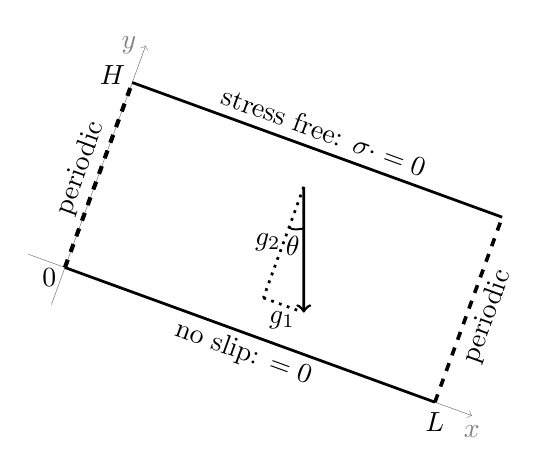
\begin{tikzpicture}[scale=2.5,rotate=-20]
  \draw[->,gray,very thin] (-0.2,0.0) -- (2.2,0.0) node[below] {$x$};
  \draw[->,gray,very thin] (0.0,-0.2) -- (0.0,1.2) node[left] {$y$};
  \node[xshift=-0.2cm,yshift=-0.13cm] at (0.0,0.0) {$0$};
  \node[xshift=0.0cm,yshift=-0.25cm] at (2.0,0.0) {$L$};
  \node[xshift=-0.25cm,yshift=0.1cm] at (0.0,1.0) {$H$};
  \draw[line width=1.0pt] (0.0,0.0) -- (2.0,0.0);
  \draw[line width=1.0pt] (0.0,1.0) -- (2.0,1.0);
  \node[rotate=-20] at (1.0,-0.1) {no slip: $\bu=0$};
  \node[rotate=-20] at (1.0,1.1) {stress free: $\sigma\cdot\bn=0$};
  \draw[line width=1.5pt,dashed] (0.0,0.0) -- (0.0,1.0);
  \draw[line width=1.3pt,dashed] (2.0,0.0) -- (2.0,1.0);
  \node[rotate=70] at (-0.1,0.5) {periodic};
  \node[rotate=70] at (2.1,0.5) {periodic};
  \draw[line width=1.0pt,dotted] (1.0,0.8) -- node[xshift=-0.2cm,yshift=0.0cm] {$g_2$} (1.0,0.2);
  \draw[line width=1.0pt,dotted] (1.0,0.2) -- node[xshift=0.0cm,yshift=-0.2cm] {$g_1$} (1.2,0.2);
  %>> 0.6 * tan((pi/180)*20)
  %ans =  0.21838
  \draw[->,line width=1.0pt] (1.0,0.8) -- (1.21838,0.2) node[xshift=0.2cm,yshift=0.6cm] {$\bg$};
  \draw[line width=0.7pt] (1.0,0.58) .. controls (1.03,0.575) and (1.04,0.585) .. (1.07,0.6);
  \node at (1.05,0.5) {$\theta$};
\end{tikzpicture}


\caption{Geometry and boundary conditions of our first Stokes problem, for sticky fluid flowing down a slope.}
\label{fig:ok:slabonslope}
\end{marginfigure}

Because the flow is actually intended to be infinite in the $x$ direction, for a numerical approximation we will require the solution to be periodic in $x$, so the domain is the rectangle $[0,L]\times[0,H]$ (in the rotated coordinates), where $H$ is the thickness and $L$ the length.  We assume a stress-free top and no slip at the base.  Because the normal direction to the top is in the (rotated) $y$-direction, the top boundary condition is
  $$\sigma\cdot\bn = 0 \iff
\begin{bmatrix}
2 \nu u_x - p & \nu (u_y+v_x) \\
\nu (u_y+v_x) & 2 \nu v_y - p
\end{bmatrix} \begin{bmatrix}
0 \\ 1
\end{bmatrix} = \begin{bmatrix}
0 \\ 0
\end{bmatrix}.$$
Thus, with the no-slip base, we have these boundary conditions,
\begin{align}
\text{top $y=H$:}&    & &\begin{array}{l} u_y + v_x = 0 \\ 2 \nu v_y = p\end{array}  \label{eq:ok:bcstokestop} \\
\text{bottom $y=0$:}& & &\begin{array}{l} u = 0 \\ v = 0 \end{array} \label{eq:ok:bcstokesbottom} \\
\text{sides $x=0$ and $x=L$:}&
                      & &u,v,p \text{ are periodic}. \label{eq:ok:bcstokesperiodic}
\end{align}

This boundary-value problem, consisting of field equations \eqref{eq:ok:stokes2du}--\eqref{eq:ok:stokes2dincomp} and boundary conditions \eqref{eq:ok:bcstokestop}--\eqref{eq:ok:bcstokesperiodic}, has a well-known exact solution, which makes this a good example for our first numerical approach:
\begin{align}
u &= \frac{g_1}{\nu} y \left(H - \frac{y}{2}\right), \label{eq:ok:exactstokesu} \\
v &= 0, \label{eq:ok:exactstokesv} \\
p &= -g_2 (H-y).\label{eq:ok:exactstokesp}
\end{align}
It is not hard to explain how this solution is derived.  First, the solution of the problem is unique by standard arguments with the weak formulation \citep[p.~223]{Elmanetal2005}.  Thus the solution is independent of $x$ because the transformation $x\mapsto x+c$ changes none of the equations or boundary conditions.  Next, by \eqref{eq:ok:stokes2du} and boundary conditions \eqref{eq:ok:bcstokestop}, \eqref{eq:ok:bcstokesbottom}, $u=u(y)$ solves the easy two-point boundary value problem $-\nu u_{yy} = g_1$, $u(0)=0$, $u_y(H)=0$ which gives \eqref{eq:ok:exactstokesu}.  But then by \eqref{eq:ok:stokes2dincomp} and the boundary condition \eqref{eq:ok:bcstokesbottom}, $v=0$.  Finally for the pressure $p=p(y)$, equations \eqref{eq:ok:stokes2dv} and \eqref{eq:ok:bcstokestop} say $p_y=g_2$ and $p(H)=0$ thus \eqref{eq:ok:exactstokesp}.


\section{Block structure and symmetry}

FIXME: Laplacians are something we understand, so lets proceed with eqns \eqref{eq:ok:stokes2du}, \eqref{eq:ok:stokes2dv}

FIXME: any way we do \eqref{eq:ok:stokes2dincomp} we get block structure for the full system ``$A \bz = \bbf$.''  Informally the structure is
  $$\begin{bmatrix}
    -\nu\grad^2 & 0 & \partial/\partial x \\
    0 & -\nu\grad^2 & \partial/\partial y \\
    -\partial/\partial x & -\partial/\partial y & 0
    \end{bmatrix}
    \begin{bmatrix}
    \bu \\ \bv \\ \bp
    \end{bmatrix}
    =
    \begin{bmatrix}
    g_1 \\ g_2 \\ 0
    \end{bmatrix}
    $$
but let's write
  $$\begin{bmatrix}
    \nu L_1 & 0 & G_1 \\
    0 & \nu L_2 & G_2 \\
    B_1 & B_2 & 0
    \end{bmatrix}
    \begin{bmatrix}
    \bu \\ \bv \\ \bp
    \end{bmatrix}
    =
    \begin{bmatrix}
    g_1 \\ g_2 \\ 0
    \end{bmatrix}
    $$
where $L_i$, $G_i$, $B_i$ are matrices.  We expect that Laplacian-approximation matrices $L_1$ and $L_2$, which essentially differ only in their boundary conditions, can be built as symmetric positive-definite matrices.

FIXME: $A$ certainly not invertible if approx to ``$\Div \bu$'' (i.e.~$\begin{bmatrix} B_1 & B_2 \end{bmatrix}$) has more rows than columns

FIXME: careful implementation of finite differences are required so as to make symmetric, i.e.~make $B_1=G_1^\top$, $B_2=G_2^\top$:
    $$\begin{bmatrix}
    \nu L_1 & 0 & G_1 \\
    0 & \nu L_1 & G_2 \\
    G_1^\top & G_2^\top & 0
    \end{bmatrix}
    \begin{bmatrix}
    \bu \\ \bv \\ \bp
    \end{bmatrix}
    =
    \begin{bmatrix}
    g_1 \\ g_2 \\ 0
    \end{bmatrix}$$
Now system is symmetric, but not positive definite.

Before proceeding let us observe that the pressure can be seen to solve its own equation, at least assuming smoothness of the solution to \eqref{eq:ok:stokes2du}--\eqref{eq:ok:stokes2dincomp}.  By taking the $x$ and $y$ derivatives of \eqref{eq:ok:stokes2dincomp} we get equations $u_{xx} + v_{yx} = 0$ and $u_{xy} + v_{yy} = 0$.  These allow us to replace $u_{xx}$ and $v_{yy}$ in \eqref{eq:ok:stokes2du}, \eqref{eq:ok:stokes2dv} with mixed derivatives, respectively, to get:
\begin{align}
-\nu \left(-v_{yx} + u_{yy}\right) + p_x &= g^x \label{eq:ok:mixedstokes2du} \\
-\nu \left(v_{xx} - u_{xy}\right) + p_y &= g^y \label{eq:ok:mixedstokes2dv}
\end{align}
Now, taking the $x$ derivative of \eqref{eq:ok:mixedstokes2du} and the $y$-derivative of \eqref{eq:ok:mixedstokes2dv}, and noting components $g^j$ are constant, and adding the results, the velocity derivatives cancel entirely.  We conclude that $p$ actually solves Laplace's equation,
\begin{equation}
\grad^2 p = 0. \label{eq:ok:pressurepoisson}
\end{equation}
The derivation here is not original; we have arrived at the well-known \emph{pressure-Poisson} equation \citep[FIXME: check]{Ockendonetal2003}.

The appearance of the Laplacian in a decoupled equation opens up the possibility that we can make our linear system ``more positive definite'' by adding a multiple of equation \eqref{eq:ok:pressurepoisson} to the Stokes system.  Concretely, if $\eps\ge 0$ then this system is equivalent to \eqref{eq:ok:stokes2du}--\eqref{eq:ok:stokes2dincomp}:
\begin{align}
-\nu \grad^2 u + p_x &= g^x \label{eq:ok:ppstokes2du} \\
-\nu \grad^2 v + p_y &= g^y \label{eq:ok:ppstokes2dv} \\
- u_x - v_y - \eps \grad^2 p &= 0 \label{eq:ok:ppstokes2dincomp}
\end{align}
These equations correspond to block structure of the numerical approximation,
\begin{equation}
\begin{bmatrix}
    \nu L_1 & 0 & G_1 \\
    0 & \nu L_1 & G_2 \\
    G_1^\top & G_2^\top & \eps L_3
    \end{bmatrix}
    \begin{bmatrix}
    \bu \\ \bv \\ \bp
    \end{bmatrix}
    =
    \begin{bmatrix}
    g^x \\ g^y \\ 0
    \end{bmatrix} \label{eq:ok:blockppstokes}
\end{equation}
which we write as $A\bz = \bbf$ for the rest of this Chapter.  We show parameters $\nu>0$ and $\eps \in \RR$ to emphasize that we can play with problems of different viscosity and with more or less pressure-Poisson regularization, respectively. 


\section{Finite element, structured-grid approach}

In this section we apply FIXME to equations \eqref{eq:ok:ppstokes2du}--\eqref{eq:ok:ppstokes2dincomp} using boundary conditions \eqref{eq:ok:bcstokestop}--\eqref{eq:ok:bcstokesperiodic} to get a symmetric linear system
\begin{equation}
  A \bz = \bbf \label{eq:ok:linsysstokes}
\end{equation}
with block structure \eqref{eq:ok:blockppstokes}.  As usual we treat the linear problem as nonlinear, and we use a structured grid, so our code has a \pSNES and \pDMDA objects.  We first provide a residual-evaluation routine for the locally-owned part of the structured grid.

FIXME: replace with $Q^2$--$Q^1$ (Taylor-Hood) finite elements:  To get started on the FD equations, and recalling the notation from Chapter \ref{chap:st}, suppose that we have a grid of \texttt{Mx} points in the $x$ direction and \texttt{My} points in the $y$ direction.  Periodicity in the $x$ direction means that there is a difference in the computation of grid spacing:
\begin{equation}
h_x = \frac{L}{\text{\texttt{Mx}}}, \qquad h_y = \frac{H}{\text{\texttt{My}}-1}. \label{eq:ok:hdefinestokes}
\end{equation}
The reason for the difference is suggested by Figure \ref{fig:ok:xperiodicgrid}, where we see that each grid point along the $x$-axis represents an entire grid cell, while in the $y$ direction the first and last grid points represent boundary locations.  Of course the main idea of periodicity is that left neighbors of $i=0$ grid locations are ``wrapped-around'' to the right-most grid points, while right neighbors of $i=\text{\texttt{Mx}}-1$ locations are wrapped to the left-most grid points.

\begin{marginfigure}
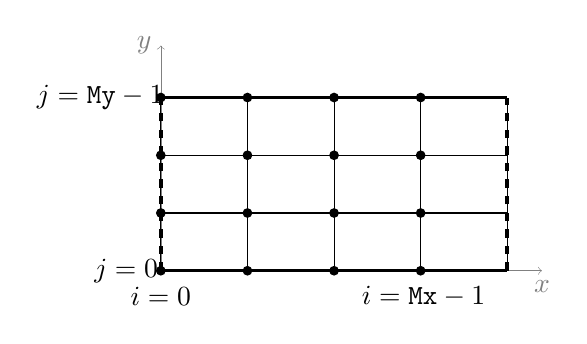
\begin{tikzpicture}[scale=2.2]
  \draw[->,gray,very thin] (0.0,0.0) -- (2.2,0.0) node[below] {$x$};
  \draw[->,gray,very thin] (0.0,0.0) -- (0.0,1.3) node[left] {$y$};
  \draw[line width=1.0pt] (0.0,0.0) -- (2.0,0.0);
  \draw[line width=1.0pt] (0.0,1.0) -- (2.0,1.0);
  \draw[line width=1.5pt,dashed] (0.0,0.0) -- (0.0,1.0);
  \draw[line width=1.3pt,dashed] (2.0,0.0) -- (2.0,1.0);
  \pgfmathsetmacro\fourth{1.0/4.0}
  \pgfmathsetmacro\third{1.0/3.0}
  \node at (0.0,-0.15) {$i=0$};
  \node at (1.85-\third,-0.15) {$i=\text{\texttt{Mx}}-1$};
  \node at (-0.2,0.0) {$j=0$};
  \node at (-0.35,1.0) {$j=\text{\texttt{My}}-1$};
  \draw[xstep=2.0*\fourth,ystep=\third,black,thin] (0.0,0.0) grid (2.0,1.0);
  \foreach \x in {0,...,3} {
    \foreach \y in {0,...,3} {
        \filldraw (\x * 2.0 * \fourth,\y * \third) circle (0.7pt);
    }
  }
\end{tikzpicture}


\caption{Because the grid is periodic in $x$, but not in $y$, the computation of $h_x$ and $h_y$ follows formulas \eqref{eq:ok:hdefinestokes}.}
\label{fig:ok:xperiodicgrid}
\end{marginfigure}

The FD equations for interior points, including the periodic boundaries, i.e.~any location $(i,j)$ where $0 < j < \text{\texttt{My}}-1$, are the approximations to equations \eqref{eq:ok:ppstokes2du}--\eqref{eq:ok:ppstokes2dincomp}:
\begin{align}
-\nu \Big(\frac{u_{i+1,j} - 2 u_{i,j} + u_{i-1,j}}{h_x^2} &+ \frac{u_{i,j+1} - 2 u_{i,j} + u_{i,j-1}}{h_y^2}\Big) \notag \\
&\qquad + \frac{p_{i+1,j}-p_{i-1,j}}{2h_x} - g_1 = 0 \label{eq:ok:fdstokes2du} \\
-\nu \Big(\frac{v_{i+1,j} - 2 v_{i,j} + v_{i-1,j}}{h_x^2} &+ \frac{v_{i,j+1} - 2 v_{i,j} + v_{i,j-1}}{h_y^2}\Big) \notag \\
&\qquad + \frac{p_{i,j+1}-p_{i,j-1}}{2h_y} - g_2 = 0 \label{eq:ok:fdstokes2dv} \\
- \frac{u_{i+1,j}-u_{i-1,j}}{2h_x} - \frac{v_{i,j+1}-v_{i,j-1}}{2h_y} &- \eps \Big(\frac{p_{i+1,j} - 2 p_{i,j} + p_{i-1,j}}{h_x^2} \notag \\
&\qquad\quad + \frac{p_{i,j+1} - 2 p_{i,j} + p_{i,j-1}}{h_y^2}\Big) = 0 \label{eq:ok:fdstokes2dincomp}
\end{align}
In the above formulas, so as to address periodicity in the $x$ direction, in the case $i=0$ we interpret an ``$i-1$'' subscript as $\text{\texttt{Mx}}-1$, while if $i=\text{\texttt{Mx}}-1$ then we interpret an ``$i+1$'' subscript as $0$.

At the bottom $y=0$ we set fields from the Dirichlet boundary conditions \eqref{eq:ok:bcstokesbottom}, and from the exact solution for $p$:
\begin{equation}
  u_{i,0} = v_{i,0} = 0, \quad p_{i,0} = - g_2 H. \label{eq:ok:fdbcstokesbottom}
\end{equation}
For the top ($y=H$) boundary conditions, let $J=\text{\texttt{My}}-1$, the upper most index in the $y$ direction.  We set $p$ from the exact solution, $p_{i,J} = 0$.

The remaining top boundary conditions \eqref{eq:ok:bcstokestop} require care.  Approximating the first of equations \eqref{eq:ok:bcstokestop} at $(x_i,y_J)$ by centered FD formulas gives
\begin{equation}
  \frac{u_{i,J+1}-u_{i,J-1}}{2h_y} + \frac{v_{i+1,J}-v_{i-1,J}}{2h_x} = 0, \label{eq:ok:earlyfdbcstokestop}
\end{equation}
but the notional point ``$u_{i,J+1}$'' is outside the domain.  We add equation \eqref{eq:ok:fdstokes2du} at the same point, solved for $u_{i,J+1}$,
\begin{equation}
  u_{i,J+1} = 2 u_{i,J} - u_{i,J-1} - h_y^2 \left(\frac{g_1}{\nu} + \frac{u_{i+1,J} - 2 u_{i,J} + u_{i-1,J}}{h_x^2}\right) \label{eq:ok:earlyfdstokes2dutop} 
\end{equation}
and incorporating $p_{i-1,J}=p_{i+1,J}=0$ also, and substitute this into \eqref{eq:ok:earlyfdbcstokestop}.

The second of equations \eqref{eq:ok:bcstokestop} says $v_y=0$ at $(x_i,y_J)$ because $p_{i,J}=0$, so $v_{i,J+1} = v_{i,J-1}$ from the centered FD approximation.  But then \eqref{eq:ok:fdstokes2dv} and \eqref{eq:ok:fdstokes2dincomp} become the pair of equations
\begin{align}
-\nu \Big(\frac{v_{i+1,J} - 2 v_{i,J} + v_{i-1,J}}{h_x^2} + \frac{2 v_{i,J-1} - 2 v_{i,J}}{h_y^2}\Big) + \frac{p_{i,J+1}-p_{i,J-1}}{2h_y} - g_2 = 0 \label{eq:ok:fdtopv} \\
\frac{u_{i+1,J}-u_{i-1,J}}{2h_x}  - \eps \frac{p_{i,J+1} + p_{i,J-1}}{h_y^2} = 0. \label{eq:ok:earlytoppressure}
\end{align}
These equations both have the notional ``$p_{i,J+1}$,'' so we eliminate it by rewriting equation \eqref{eq:ok:earlytoppressure},
\begin{equation}
p_{i,J+1} = \frac{h_y^2}{\eps} \frac{u_{i+1,J}-u_{i-1,J}}{2h_x} - p_{i,J-1},\label{eq:ok:fdtoppressureelim}
\end{equation}
which is substituted into \eqref{eq:ok:fdtopv}.

FIXME: the resulting code is \texttt{stokes.c}


\section{Preconditioners for indefinite systems}

FIXME: while $A$ is symmetric, it is not positive definite; note that if
    $$M = \begin{bmatrix} 0 & G \\ G^\top & 0 \end{bmatrix}$$
and if $M$ has eigenvalue $\lambda$ so that
    $$M \begin{bmatrix} \bx \\ \by \end{bmatrix} = \lambda \begin{bmatrix} \bx \\ \by \end{bmatrix}$$
then
    $$M \begin{bmatrix} -\bx \\ \by \end{bmatrix} = - \lambda \begin{bmatrix} -\bx \\ \by \end{bmatrix}$$
and (w.o.l.o.g.) this is a lin.-indep. eigenvector so $M$ also has eigenvalue $-\lambda$


\section{Exercises}

\renewcommand{\labelenumi}{\arabic{chapter}.\arabic{enumi}\quad}
\begin{enumerate}

\item \label{exer:ok:constantviscositystokes}  Starting from \eqref{eq:ok:gradudefinition}, by commuting mixed derivatives and using incompressibility show that
\begin{equation*}
\Div \left(\grad \bu^{\top}\right) = \begin{bmatrix}
    \frac{\partial}{\partial x}\left(\Div \bu\right) & \frac{\partial}{\partial y }\left(\Div \bu\right) & \frac{\partial}{\partial x} \left(\Div \bu\right)
    \end{bmatrix}
    = 0.
\end{equation*}
On the other hand,
\begin{equation*}
\Div \left(\grad \bu\right) = \begin{bmatrix} \grad^2 u^x & \grad^2 u^y & \grad^2 u^z \end{bmatrix} = \grad^2 \bu.
\end{equation*}
defines the symbol ``$\grad^2 \bu$.''  Thereby we derive \eqref{eq:ok:constantviscositystokes}
%\item FIXME: apply chapter 2 idea of making more symmetric boundary conditions

\item \label{exer:ok:smalldetails}  FIXME
%f_0 = - \int_\Omega \grad \psi_{-1} \cdot \grad \psi_0
%g_0 = \int_{\square_0} \partial \psi_{-1}/\partial x
%g_2 = \int_{\square_2} \partial \psi_{-1}/\partial x

\end{enumerate}
